\documentclass[a4paper, 12pt]{article}

% Русский язык
\usepackage[T2A]{fontenc}
\usepackage[utf8]{inputenc}
\usepackage[english,russian]{babel}

% Картинки
\usepackage{graphicx}
\graphicspath{{images/}}
\DeclareGraphicsExtensions{.pdf,.png,.jpg}
\usepackage{wrapfig}

% Математика
\usepackage{amsmath,amsfonts,amssymb,amsthm,mathtools} 

% Параметры страницы
\usepackage[left=2cm,right=2cm,top=2cm,bottom=3cm,bindingoffset=0cm]{geometry}

\usepackage{enumitem,xparse}
\usepackage{caption}
\usepackage{subcaption}
\usepackage{float}

\usepackage{listings}
\usepackage{xcolor}
\lstset{
  language=C++,
  backgroundcolor=\color{gray!5},
  basicstyle=\ttfamily\small,
  numbers=left,
  numberstyle=\tiny\color{gray},
  frame=single,
  rulecolor=\color{black!30},
  breaklines=true,
  keywordstyle=\color{blue}\bfseries,
  commentstyle=\color{green!50!black}\itshape,
  stringstyle=\color{orange},
  showstringspaces=false,
  tabsize=2
}

\begin{document}

\newgeometry{left=2cm,right=2cm,top=2cm,bottom=1cm,bindingoffset=0cm}
\begin{titlepage}
    
    \begin{center}
        \vspace*{5cm}
        \Huge Московский Физико-Технический Институт
        \vspace*{2cm}\\
        \\\vspace*{0.25cm}
        
        \noindent\rule{\textwidth}{1pt}
        \vspace*{-0.25cm}
        
        \huge \textbf{Лаба по флоатам}
        \noindent\rule{\textwidth}{1pt}

        \vspace{6cm}
       \vfill
        \begin{flushright}
            \begin{minipage}{.4\textwidth}
            \Large Выполнил:\\ Студент 1 курса ФАКТ\\ Группа Б03-504 \\Подмосковнов Лев\\
            \end{minipage}
        \end{flushright}
        
        \vfill
        \normalsize Долгопрудный \\2025
        
    \end{center}
\end{titlepage}
\restoregeometry

\setcounter{page}{2}

\subsection*{0. unsigned int -> binary}

\begin{lstlisting}
void ui_to_bin(unsigned int a) {
    for (int i = 32 - 1; i >= 0; i--) {
        cout << ((a >> i) & 1);
        if (i != 0 && i % 8 == 0) {
            cout << " ";
        }
    }
}
\end{lstlisting}



Функция для перевода и печати в двоичную систему переменную типа unsigned int.

\subsection*{1. float -> binary}

\begin{lstlisting}
union fu {
 float f;
 unsigned int u;
};

void ui_to_bin(unsigned int a) {
    for (int i = 32 - 1; i >= 0; i--) {
        cout << ((a >> i) & 1);
        if (i == 31 || i == 23) {
            cout << "|";
        }
        if (i != 0 && i % 4 == 0) {
            cout << " ";
        }
    }
}
\end{lstlisting}

В структуру fu записываем в f наше число. Теперь нужно посмотреть на биты float через unsigned int.

\subsection*{2. Переполнение мантисы}

В ходе эксперимента найдено, что последняя степень 10, которая не переполняет мантису 11. Когда хотим положить в float $2^{12}$ получается число 99999997952.00.


\subsection*{3. Бесконечный цикл}

В ходе эксперимента было замечено, что к число 16777216.0 в float нельзя добавить единицу.

\newpage

\subsection*{4. Численное интегрирование}

\begin{figure}[h]
    \centering
    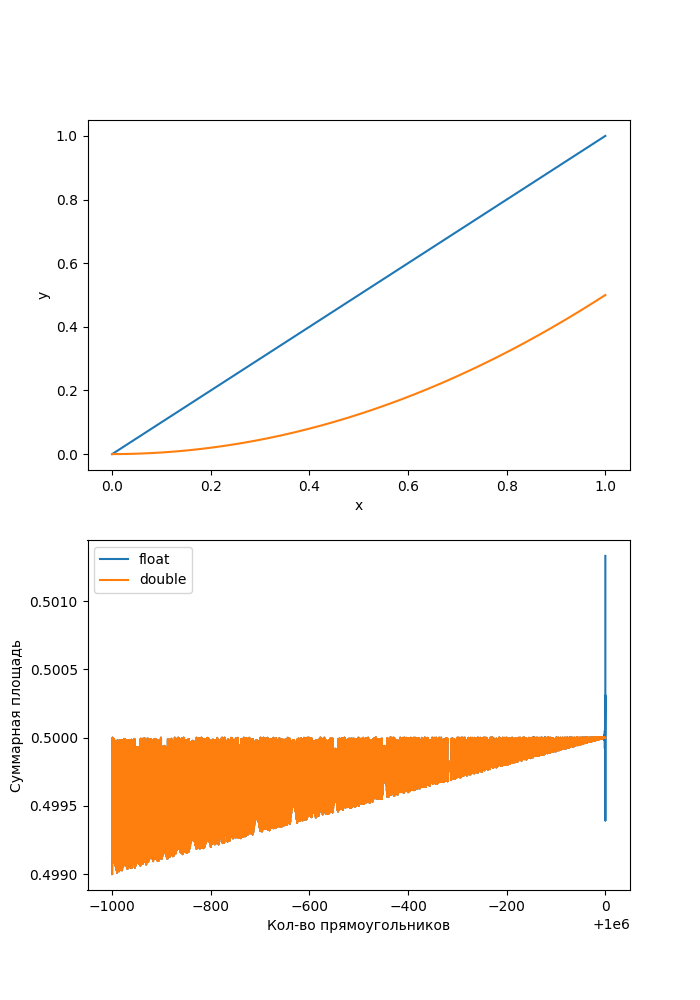
\includegraphics[width=0.7\textwidth]{4.png}
\end{figure}

При увелечении количества столбцов результат становится точнее и в float, и в double. Float ломается быстрее чем double.

\newpage

\subsection*{5*. Антипереполнение}

Subnormal / denormal — это числа с очень маленьким модулем, которые находятся между нулём и самым маленьким нормальным числом IEEE-754. Они имеют нулевой (biased) экспонент-поле и ненулевую мантиссу; обеспечивают плавное (gradual) антипереполнение. Без них некоторые разности могли бы сразу дать 0.

Underflow (антипереполнение) — ситуация, когда результат арифметики меньше минимального нормального значения. С появлением subnormals результат может быть subnormal (потеря точности), а без них — прямо 0.

DAZ (Denormals-Are-Zero) — если входной операнд (операнты) является денормалом, он заменяется на ноль до выполнения операции (то есть входные денормалы “приравниваются к 0”).

FTZ (Flush-To-Zero) — если результат операции получился денормалом, вместо него возвращается 0.

При DAZ/FTZ OFF вы часто увидите, что операция с денормалами значительно медленнее

\end{document}